\documentclass[11pt,a4paper]{article}

\usepackage[margin=2.5cm]{geometry}
\usepackage[T1]{fontenc}
\usepackage{lmodern}
\usepackage{microtype}
\usepackage{booktabs}
\usepackage{longtable}
\usepackage{xcolor}
\usepackage{listings}
\usepackage{amsmath}
\usepackage{amssymb}
\usepackage{enumitem}
\usepackage{tikz}
\usetikzlibrary{arrows.meta,positioning}
\usepackage[hidelinks]{hyperref}

\definecolor{codebg}{RGB}{247,247,247}
\definecolor{codekey}{RGB}{20,80,160}
\definecolor{codestr}{RGB}{150,60,20}

\lstdefinestyle{json}{
  basicstyle=\ttfamily\footnotesize,
  backgroundcolor=\color{codebg},
  breaklines=true, columns=fullflexible, keepspaces=true,
  showstringspaces=false, frame=single, framerule=0pt, framesep=6pt,
  xleftmargin=6pt, stringstyle=\color{codestr},
  literate=*{:}{{{\color{codekey}:}}}{1}{\{}{{{\color{codekey}\{}}}{1}{\}}{{{\color{codekey}\}}}}{1},
}
\lstdefinestyle{plain}{
  basicstyle=\ttfamily\footnotesize, backgroundcolor=\color{codebg},
  breaklines=true, columns=fullflexible, keepspaces=true,
  showstringspaces=false, frame=single, framerule=0pt, framesep=6pt, xleftmargin=6pt,
}
\lstset{style=json}

\newcommand{\code}[1]{\texttt{\small #1}}
\newcommand{\file}[1]{\texttt{\small #1}}

% ---- GitHub links to the shipped example models -------------------------------
\newcommand{\ghbase}{https://github.com/ArashMassoudieh/OpenHydroQual/blob/master}
\newcommand{\ghtree}{https://github.com/ArashMassoudieh/OpenHydroQual/tree/master}
% \exfile{path relative to the repository root}
\newcommand{\exfile}[1]{\href{\ghbase/#1}{\file{#1}}}
% \exdir{path relative to the repository root}
\newcommand{\exdir}[1]{\href{\ghtree/#1}{\file{#1}}}

\title{\textbf{Plant Water Uptake in OpenHydroQual}\\[0.3em]
       \large Transpiration sources and the demand-driven crop block}
\author{}
\date{}

\begin{document}
\maketitle
\vspace{-2.5em}

\begin{abstract}
\noindent
OpenHydroQual offers two ways to take water out of a soil profile through
plants. The first attaches a transpiration \emph{source} to each soil layer and
scales a reference evapotranspiration by a crop coefficient, a stress function
and a per-layer root fraction that the user supplies. The second introduces a
\emph{crop block} that owns the atmospheric demand, and one \emph{uptake link}
per soil layer that derives its own root fraction from the geometry of the
profile and redistributes demand away from layers that have dried out. This
document sets out both formulations, states precisely what each can and cannot
represent, and documents the components and their parameters. The models
referenced throughout are in the repository and are linked as they arise.
\end{abstract}

\tableofcontents

% ==============================================================================
\section{Scope and the choice between the two models}
% ==============================================================================

Everything in this document concerns \emph{transpiration}: water taken up by
roots and lost through stomata. Evaporation directly from the soil surface is a
separate process and is left to the \code{Evapotranspiration\_*(Soil)} sources.
The crop coefficients used here are FAO-56 \emph{basal} coefficients $K_{cb}$,
which exclude soil evaporation by definition, so the two can be added without
double counting.

The two models differ in where the demand lives.

\begin{description}[leftmargin=1.4cm,style=nextline]
\item[Model 1, transpiration sources] A source is attached to each soil layer.
  It computes that layer's transpiration directly from a reference
  evapotranspiration, a crop coefficient, a stress coefficient evaluated on the
  layer's own moisture state, and a root fraction that the user types in. The
  layers do not know about one another. If one dries out, its share of the
  transpiration is simply lost.
\item[Model 2, crop block and uptake links] A \code{Crop} block computes a
  single potential transpiration for the whole plant. One
  \code{Root\_uptake\_link} per layer carries a share of that demand. The shares
  are derived from the profile geometry rather than entered, and a compensation
  mechanism lets layers that are still wet make up for layers that are stressed.
\end{description}

Model 1 is the lighter of the two and is adequate when the profile stays
reasonably uniform or when the root distribution is genuinely known and fixed.
Model 2 is what you want when the profile dries unevenly, when roots grow
during a season, or when you care about the difference between potential and
actual transpiration.

Both live in \exfile{resources/plants.json}.

% ==============================================================================
\section{Model 1: transpiration sources}
% ==============================================================================

\subsection{Formulation}

For a soil layer $i$,
\begin{equation}
T_i \;=\; ET_0 \; K_{cb} \; K_s(\theta_i) \; f_i \; A ,
\end{equation}
where $ET_0$ is the reference evapotranspiration, $K_{cb}$ the basal crop
coefficient, $K_s$ a water stress coefficient in $[0,1]$, $f_i$ the fraction of
the root system in this layer and $A$ the layer's plan area.

The stress coefficient is a linear ramp in effective saturation between the
pressure heads corresponding to field capacity and permanent wilting point. In
terms of the van Genuchten parameters that the \code{Soil} block already
exposes,
\begin{equation}
K_s \;=\; \min\!\left(
  \frac{S_e - S_e(h_{\mathrm{wp}})}{S_e(h_{\mathrm{fc}}) - S_e(h_{\mathrm{wp}})},\; 1
\right)^{\!+},
\qquad
S_e(h) = \bigl(1+(\alpha h)^n\bigr)^{-m},
\end{equation}
evaluated at $h_{\mathrm{fc}} = 3.3$~m and $h_{\mathrm{wp}} = 150$~m of suction.
The superscript $+$ denotes clipping at zero.

\subsection{Why the depletion fraction $p$ is not available here}

The full FAO-56 stress function introduces a crop-specific readily available
water fraction $p$, so that $K_s = 1$ until depletion exceeds $p\,\mathrm{TAW}$
and falls linearly thereafter. That form is not expressible as a source in
OpenHydroQual, and the reason is worth stating because it is a genuine
structural limit rather than an oversight.

A source computes its contribution as
\[
  \text{value} \;=\; \text{coefficient} \times \text{timeseries} \times \text{rate},
\]
where \code{coefficient} is evaluated \emph{against the block} it is attached
to, and \code{rate} and \code{timeseries} are evaluated \emph{against the
source}. A block expression can see the soil state but not the source's
parameters; a source expression can see its own parameters but not the soil
state. The FAO-56 $K_s$ mixes the two inside a single $\min(\cdot)$, so it can
be written in neither place. Setting $p = 0$ recovers the linear ramp above,
which is what these sources implement.

Model 2 does not have this restriction, because a link expression can read both
of its endpoints. The Feddes function in Section~\ref{sec:feddes} is the full
four-parameter form.

\subsection{Components}

\begin{longtable}{@{}p{5.0cm}p{9.5cm}@{}}
\toprule
\textbf{Type} & \textbf{Purpose} \\
\midrule
\endhead
\code{Transpiration\_Time\_Series (Soil)} &
  $ET_0$ supplied as a time series. \\
\code{Transpiration\_Penman (Soil)} &
  $ET_0$ computed internally from solar radiation, air temperature, relative
  humidity and wind speed. \\
\bottomrule
\end{longtable}

\noindent
Both take \code{Kcb} and \code{root\_fraction}. Attach one to each soil layer's
\code{Evapotranspiration} property and make the root fractions sum to one
yourself; nothing checks this for you.

\subsection{Examples}

\begin{itemize}[leftmargin=1.4cm]
\item \exfile{Examples/Plant\_Transpiration/rooted\_soil\_profile.ohq} --- three
  soil layers with root fractions $0.5/0.3/0.2$ and $ET_0$ from a time series.
\item \exfile{Examples/Plant\_Transpiration/rooted\_soil\_profile\_penman.ohq}
  --- the same profile with $ET_0$ computed by the Penman combination equation
  from half-hourly weather observations.
\end{itemize}

\noindent
The folder is \exdir{Examples/Plant\_Transpiration}.

% ==============================================================================
\section{Model 2: the crop block and root uptake links}
% ==============================================================================

\subsection{Structure}

\begin{center}
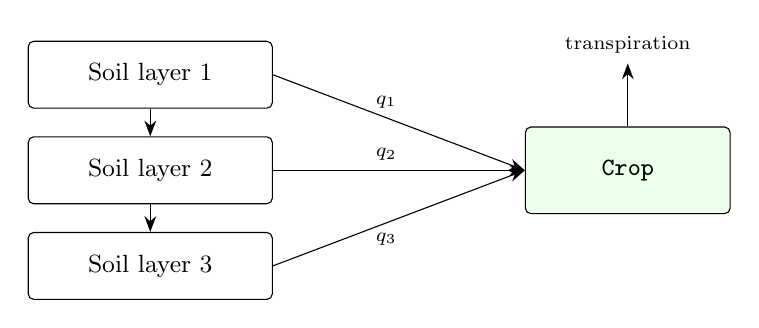
\begin{tikzpicture}[
  blk/.style={draw,rounded corners=2pt,minimum width=3.1cm,minimum height=0.85cm,font=\small},
  crop/.style={draw,rounded corners=2pt,fill=green!8,minimum width=2.6cm,minimum height=1.1cm,font=\small},
  >={Stealth[length=2mm]}]
\node[blk] (l1) {Soil layer 1};
\node[blk,below=0.35cm of l1] (l2) {Soil layer 2};
\node[blk,below=0.35cm of l2] (l3) {Soil layer 3};
\node[crop,right=3.2cm of l2] (c) {\code{Crop}};
\draw[->] (l1.east) -- node[above,font=\scriptsize,pos=0.45] {$q_1$} (c.west);
\draw[->] (l2.east) -- node[above,font=\scriptsize,pos=0.45] {$q_2$} (c.west);
\draw[->] (l3.east) -- node[below,font=\scriptsize,pos=0.45] {$q_3$} (c.west);
\draw[->] (c.north) -- ++(0,0.8) node[above,font=\scriptsize] {transpiration};
\draw[->] (l1.south) -- (l2.north);
\draw[->] (l2.south) -- (l3.north);
\end{tikzpicture}
\end{center}

The crop holds a small storage that represents the plant water pathway. Uptake
links fill it; transpiration empties it with a short residence time
\code{K\_plant}. The storage exists so that supply and demand balance
dynamically rather than instantaneously; it is not meant to represent plant
water content.

\subsection{Atmospheric demand}

\begin{equation}
T_p \;=\; ET_0 \; K_{cb} \; f_c \; A ,
\qquad
f_c \;=\; 1 - e^{-k\,\mathrm{LAI}} .
\end{equation}

The cover fraction $f_c$ is Beer's law with extinction coefficient $k$ (about
$0.6$ for most field crops), so the transpiring fraction of the surface follows
canopy development rather than being assumed. Leaf area index is
\begin{equation}
\mathrm{LAI} \;=\; \mathrm{LAI}_{\text{constant}} + \mathrm{LAI}_{\text{series}},
\end{equation}
so a static canopy needs only the constant and a seasonal canopy needs only the
series. The rooting depth is composed the same way.

\subsection{Root distribution}

Root density falls off exponentially with depth,
\begin{equation}
\rho(z) \;\propto\; e^{-\lambda z / Z_r}, \qquad 0 \le z \le Z_r ,
\end{equation}
with $Z_r$ the rooting depth and $\lambda$ a shape parameter. Small $\lambda$
approaches a uniform distribution; $\lambda \approx 2$ is typical.

Each uptake link integrates this density over its own layer. The link reads the
depths to the top and bottom of the layer from the layer's
\code{bottom\_elevation} and \code{depth} and the crop's
\code{surface\_elevation}, clipping both at the root tip:
\begin{equation}
z_{\text{top}} = \min\bigl(\,(E_s - E_b - d)^+,\; Z_r \bigr),
\qquad
z_{\text{bot}} = \min\bigl(\,(E_s - E_b)^+,\; Z_r \bigr),
\end{equation}
and then
\begin{equation}
\beta \;=\; \frac{e^{-\lambda z_{\text{top}}/Z_r} - e^{-\lambda z_{\text{bot}}/Z_r}}
                 {1 - e^{-\lambda}} .
\label{eq:beta}
\end{equation}

Two properties of \eqref{eq:beta} matter in practice. Because the denominator
normalises the density over $[0, Z_r]$, the $\beta$ of a set of contiguous
layers spanning the whole root zone sums to one without the user doing
anything. And because the clipping is per-link, a layer that the root tip
reaches only partway into gets exactly the share of the root system that lies
inside it. A layer entirely below the root tip gets $\beta = 0$ and drops out
of its own accord.

Nothing here has to be entered by hand, and nothing has to be revised when a
layer is added, a layer thickness is edited, or the roots grow during a season.

\subsection{Water stress}
\label{sec:feddes}

Each link reduces its share by the Feddes stress function, evaluated on its own
layer's pressure head $h$:
\begin{equation}
\alpha(h) \;=\;
\left[
\min\!\left(
  \min\!\left(\frac{h - h_4}{h_3 - h_4},\; 1\right),\;
  \frac{h - h_1}{h_2 - h_1}
\right)
\right]^{+} .
\end{equation}
The four heads are the anoxia limit $h_1$, the wet end of the optimal range
$h_2$, the dry end of the optimal range $h_3$, and the wilting point $h_4$, all
negative and ordered $h_1 > h_2 > h_3 > h_4$. Uptake is at its full share
between $h_2$ and $h_3$, ramps down towards zero at the wilting point, and also
ramps down towards zero as the layer approaches saturation, which is the
waterlogging limb.

\begin{longtable}{@{}llrl@{}}
\toprule
\textbf{Symbol} & \textbf{Property} & \textbf{Default (m)} & \textbf{Meaning} \\
\midrule
\endhead
$h_1$ & \code{h\_anoxic}        & $-0.1$  & uptake stops above this (anoxia) \\
$h_2$ & \code{h\_optimal\_wet}  & $-0.25$ & wet end of the optimal range \\
$h_3$ & \code{h\_optimal\_dry}  & $-5$    & dry end of the optimal range \\
$h_4$ & \code{h\_wilting}       & $-160$  & permanent wilting point \\
\bottomrule
\end{longtable}

\subsection{Compensation}

Without compensation, layer $i$ delivers $T_p\,\beta_i\,\alpha_i$ and the
shortfall in a dry layer is lost. Actual transpiration is then
$T_p \sum_i \beta_i \alpha_i$, which can be far below potential even when the
profile as a whole holds plenty of water.

Real root systems do not behave that way: uptake shifts towards whatever part
of the profile can still supply. SWAP and APEX both model this. The
implementation here scales every layer by a common factor so that the total
returns to the potential rate,
\begin{equation}
q_i \;=\; T_p \, \beta_i \, \alpha_i \, C ,
\qquad
C \;=\; \frac{1}{\sum_j \beta_j \alpha_j} ,
\end{equation}
which gives $\sum_i q_i = T_p$ whenever any rooted layer can supply.

\subsubsection*{Obtaining the sum without knowing the layer count}

$C$ needs $\sum_j \beta_j \alpha_j$, a sum over the crop's links, but a block
expression can only take the \emph{average} of a quantity over its links, via
the \code{.v} suffix. A sum would need the number of links, which the block does
not know and which the user should not have to supply.

The way around it uses \eqref{eq:beta}. Since the root fractions sum to one over
a complete profile, $\overline{\beta} = 1/N$ and therefore $N =
1/\overline{\beta}$, so
\begin{equation}
\sum_j \beta_j \alpha_j
  \;=\; N \, \overline{\beta\alpha}
  \;=\; \frac{\overline{\beta\alpha}}{\overline{\beta}} ,
\end{equation}
which is two link averages and a division. In the template this is
\begin{lstlisting}[style=plain]
sum_beta_alpha      = beta_alpha.v/(beta.v+0.000000001)
compensation_factor = 1/(compensation*_max(sum_beta_alpha;0.001)+(1-compensation))
\end{lstlisting}
and it self-corrects for however many uptake links are drawn. The
\code{compensation} property switches the mechanism off by collapsing the factor
to one.

\subsubsection*{The compensation is unlimited}

$C$ is not capped. As a profile dries, $\sum_j \beta_j \alpha_j$ falls and $C$
grows without bound, concentrating the entire demand on whichever layer is still
wet; values around ten are reached in the worked example below. This is the
behaviour of full compensation as SWAP and APEX describe it, but some
implementations impose a ceiling. If you need one, the practical levers are to
raise $h_4$ so that layers reach $\alpha = 0$ sooner, or to switch compensation
off.

\subsection{Components}

\begin{longtable}{@{}p{4.2cm}p{10.3cm}@{}}
\toprule
\textbf{Type} & \textbf{Purpose} \\
\midrule
\endhead
\code{Crop} & Plant block; $ET_0$ supplied as a time series. \\
\code{Crop\_Penman} & Plant block; $ET_0$ computed internally by the Penman
  combination equation from solar radiation, air temperature, relative humidity
  and wind speed. \\
\code{Root\_uptake\_link} & Draw from a soil layer to a crop. Carries that
  layer's share of the demand. \\
\bottomrule
\end{longtable}

\subsubsection*{Crop properties}

\begin{longtable}{@{}p{4.3cm}p{2.0cm}p{8.2cm}@{}}
\toprule
\textbf{Property} & \textbf{Default} & \textbf{Meaning} \\
\midrule
\endhead
\code{area}                    & 10000  & ground area covered by the plant \\
\code{surface\_elevation}      & 0      & datum from which root depths are measured \\
\code{LAI\_constant}           & 3      & constant part of the leaf area index \\
\code{LAI\_timeseries}         & ---    & seasonal part, added to the constant \\
\code{k\_extinction}           & 0.6    & Beer's law canopy extinction coefficient \\
\code{Kcb}                     & 1.0    & FAO-56 basal crop coefficient \\
\code{root\_depth\_constant}   & 1.0    & constant part of the rooting depth \\
\code{root\_depth\_timeseries} & ---    & seasonal part, added to the constant \\
\code{root\_lambda}            & 2.0    & root density shape parameter \\
\code{h\_anoxic} \dots \code{h\_wilting} & see above & Feddes parameters \\
\code{compensation}            & 1      & 1 enables compensation, 0 disables it \\
\code{K\_plant}                & 0.01 d & residence time of the canopy pathway \\
\bottomrule
\end{longtable}

\subsubsection*{Outputs worth plotting}

\begin{longtable}{@{}p{4.6cm}p{10.0cm}@{}}
\toprule
\textbf{Quantity} & \textbf{Meaning} \\
\midrule
\endhead
\code{Tp}                     & potential transpiration, m$^3$/day \\
\code{soil\_stress}           & $\sum_j \beta_j \alpha_j$, the root-weighted water availability \\
\code{relative\_transpiration}& actual over potential transpiration \\
\code{cover\_fraction}        & $1 - e^{-k\,\mathrm{LAI}}$ \\
\code{LAI}, \code{root\_depth}& the composed canopy and root state \\
\code{beta}, \code{alpha}, \code{flow} & on each link: root share, stress, uptake \\
\code{z\_top}, \code{z\_bottom}& on each link: the depth interval it integrated over \\
\bottomrule
\end{longtable}

\noindent
Use \code{soil\_stress} as the crop stress index. With compensation on, total
uptake equals $T_p$ by construction, so \code{relative\_transpiration} sits at
one apart from the lag of the canopy reservoir, which makes it a noisy
diagnostic; it is informative when \code{compensation} is zero.
\code{soil\_stress} carries no lag.

\subsection{Two rules to observe}

\begin{enumerate}[leftmargin=1.4cm]
\item \textbf{Attach only uptake links to a crop block.} The compensation factor
  is built from \code{beta.v} and \code{beta\_alpha.v}, which average over
  \emph{all} of the block's links. Any other link type attached to a
  \code{Crop} corrupts the denominator.
\item \textbf{Do not wrap the soil layers in a composite.} A composite exposes
  one attachment point per link type per direction, so a composite containing
  the soil layers could accept only one uptake link. The crop and its layers
  must be wired individually.
\end{enumerate}

\subsection{Examples}

\subsubsection*{Root water compensation, side by side}

\exfile{Examples/Crop\_Root\_Uptake/crop\_root\_uptake.ohq} places two identical
1.5~m profiles under the same weather, differing only in the crop's
\code{compensation} setting. Rain falls for the first 15 days and then stops for
135 days. At the end of the drought:

\begin{center}
\begin{tabular}{@{}lrr@{}}
\toprule
 & \textbf{compensation on} & \textbf{compensation off} \\
\midrule
\code{soil\_stress}                        & 0.084 & 0.587 \\
$\sum q_i$ / $T_p$ \; (m$^3$/day)          & 21.9 / 21.9 & 12.9 / 21.9 \\
$\theta$, layer 1 (0.0--0.3 m)             & 0.100 & 0.107 \\
$\theta$, layer 2 (0.3--0.7 m)             & 0.100 & 0.141 \\
$\theta$, layer 3 (0.7--1.5 m)             & 0.119 & 0.184 \\
profile storage (m$^3$)                    & 1655  & 2354 \\
\bottomrule
\end{tabular}
\end{center}

The compensated crop has drawn the whole profile down to wilting point and is
still meeting its full demand, taking 98\% of it from the deepest layer. The
uncompensated crop is held at 59\% of potential although its profile still
holds 700~m$^3$ more water, because most of its root mass sits in layers that
have dried out.

The rooting depth is 1.0~m against a 1.5~m profile, so the third layer is
clipped: its \code{z\_bottom} reports 1.0~m and its $\beta$ is 0.129 rather
than the 0.229 the full layer would carry. The three $\beta$ still sum to
1.000000.

\subsubsection*{A corn season with measured weather}

\exfile{Examples/Crop\_Root\_Uptake/crop\_growing\_season\_penman.ohq} runs a
four-layer profile under a \code{Crop\_Penman} block from 1 April to 1 October
2010, with half-hourly observed solar radiation, temperature, humidity and wind.
Leaf area index is driven from a crop calendar (0 at planting, 5.0 in early
July, 0.5 at harvest) and the rooting depth grows from 0.2~m to 1.2~m over the
same period.

\begin{center}
\begin{tabular}{@{}lrrrrr@{}}
\toprule
\textbf{Date} & \textbf{LAI} & \textbf{$Z_r$ (m)} & \textbf{$ET_0$} & \textbf{$T_p$} & \textbf{$\sum\beta$} \\
\midrule
17 May & 1.74 & 0.55 & 13.3 & \phantom{0}9.9 & 1.000000 \\
16 Jul & 4.97 & 1.20 & 14.3 & 15.6 & 1.000000 \\
14 Sep & 2.04 & 1.20 & 12.9 & 10.5 & 1.000000 \\
\bottomrule
\end{tabular}
\end{center}

\noindent
Rates are instantaneous, in mm/day, sampled mid-afternoon. The root fractions
sum to one at every stage while the rooting front advances, and the share of
each layer migrates downwards as the roots grow: the topsoil link holds 0.600
of the root system in May and 0.328 in July, without any of that being entered.
Drainage to the water table is negative through the summer, which is capillary
rise supporting the crop from below.

\medskip
\noindent
\textbf{A caution on the Penman radiation term.} The Penman formulation in
OpenHydroQual drives the radiation term with incoming shortwave radiation rather
than net radiation, so it overestimates $ET_0$ by roughly a factor of two on
clear days. This example sets \code{solar\_scale\_fact} to 0.5 to compensate;
that property is the intended calibration knob and should be set from site data
before the model is used quantitatively. The same caution applies to
\code{Transpiration\_Penman (Soil)} in Model 1 and to the stock
\code{Evapotranspiration\_Penman} sources.

\medskip
\noindent
Both models, the forcing data and a fuller commentary are in
\exdir{Examples/Crop\_Root\_Uptake}.

% ==============================================================================
\section{Adding soil evaporation}
% ==============================================================================

Neither model evaporates water from the soil surface. To add it, attach an
\code{Evapotranspiration\_*(Soil)} source to the top layer. Because $K_{cb}$ is
a basal coefficient, the transpiration and evaporation terms are additive and
no double counting arises.

One caveat applies to the time-series variant. The source value is formed as
\code{coefficient} $\times$ \code{timeseries} $\times$ \code{rate}, and
\code{Evapotranspiration\_Time\_Series (Soil)} defines its \code{rate} as
\code{corr\_fact*timeseries}, so the supplied series enters the product twice
and the resulting flux is proportional to its square. Neither of the examples in
Section~5.5 uses that source. If you need a time-series soil evaporation, the
correct \code{rate} is \code{corr\_fact} alone.

% ==============================================================================
\section{Summary of the components}
% ==============================================================================

\begin{longtable}{@{}p{4.6cm}p{1.7cm}p{8.2cm}@{}}
\toprule
\textbf{Type} & \textbf{Kind} & \textbf{Notes} \\
\midrule
\endhead
\code{Transpiration\_Time\_Series (Soil)} & source & Model 1; $ET_0$ from a series;
  user supplies \code{root\_fraction} \\
\code{Transpiration\_Penman (Soil)} & source & Model 1; $ET_0$ from weather \\
\code{Crop} & block & Model 2; $ET_0$ from a series \\
\code{Crop\_Penman} & block & Model 2; $ET_0$ from weather \\
\code{Root\_uptake\_link} & link & Model 2; soil layer $\rightarrow$ crop \\
\code{Plant} & block & legacy soil--plant--atmosphere continuum block \\
\code{Soil\_to\_plant\_link} & link & legacy, used with \code{Plant} \\
\bottomrule
\end{longtable}

\noindent
All are defined in \exfile{resources/plants.json}.

\end{document}
